% !TeX TXS-program:compile = txs:///pdflatex/[--shell-escape]
\documentclass[../../../00.FullDoc/tex/ThesisSkeleton-draft2]{subfiles}

%\documentclass[12pt,a4paper,notitlepage,
%draft,
%bibliography=totoc,
%numbers=endperiod,
%appendixprefix=true,
%usenames,dvipsnames]{scrartcl} 
%\usepackage[autooneside=false, draft=false]{scrlayer-scrpage}
%\usepackage{ifdraft} %allows commands dependent on draft status
%\usepackage{scrhack}
%\usepackage{kpfonts}
%\usepackage[dvipsnames]{xcolor} %general colours
%\usepackage{colortbl} % colour for excel tables
%\usepackage{hyperref}
%\usepackage[inline]{enumitem} %inline/horizontal lists
%\hypersetup{
%	draft=true,
%	final=true,
%	colorlinks=true,
%	linktoc=all,
%	linkcolor=MidnightBlue,
%	citecolor=blue
%	%	allcolors=black
%}
%\usepackage{mwe}
%\usepackage{tipa} %IPA
%\usepackage{phonrule} %phonological rules
%\usepackage{amsmath}
%\usepackage{amsfonts}
%\usepackage{soul}
%\usepackage{amssymb}
%\usepackage{graphicx} %insert graphics, pdf etc.
%\usepackage{caption}
%\usepackage{setspace}
%\usepackage{nameref}
%\usepackage{pdfpages}
%\usepackage{csvsimple}
%\usepackage{booktabs, multicol, multirow}
%\usepackage{array}
%\usepackage{float} % float 
%\usepackage[section]{placeins}
%\usepackage{array}
%\usepackage[section]{placeins}
%\usepackage[round]{natbib} %citation package
%\bibliographystyle{agsm}
%\renewcommand{\harvardurl}{\textbf{URL:} \url}
%\usepackage{scrlayer-scrpage}
%\usepackage{blindtext}% dummy text
%\usepackage{subfiles} %subfile functionality
%\usepackage{csvsimple} %import csv tables
%\usepackage{pdflscape} %allow landscape pages
%\usepackage[inkscapearea=page]{svg}
%\usepackage[titletoc,title]{appendix}
%%\usepackage[marginpar]{todo}
%\usepackage[obeyDraft]{todonotes} %to do notes obedyDraft means not parsed if not draft
%\usepackage{etoolbox}
%%\usepackage{amsthm} % examples
%%\apptocmd{\sloppy}{\hbadness 10000\relax}{}{} %fix overfull/underfull hbox errors
%\usepackage[scaled]{helvet} 
%\renewcommand\familydefault{\sfdefault} 
%\usepackage[T1]{fontenc}
%\usepackage{listings}
%\usepackage{layouts}
%\usepackage{gb4e} %numbered examples - must be last package in preamble
%
%
%%keep figure in section & subsection
%\let\Oldsection\section
%\renewcommand{\section}{\FloatBarrier\Oldsection}
%
%\let\Oldsubsection\subsection
%\renewcommand{\subsection}{\FloatBarrier\Oldsubsection}
%
%\let\Oldsubsubsection\subsubsection
%\renewcommand{\subsubsection}{\FloatBarrier\Oldsubsubsection}
%
%%listings setup
%\lstloadlanguages{R}
%\lstset{ 
%	language=R,                     % the language of the code
%	basicstyle=\normalsize, % the size of the fonts that are used for the code
%	numbers=none,                   % where to put the line-numbers
%	numberstyle=\tiny\color{Blue},  % the style that is used for the line-numbers
%	stepnumber=1,                   % the step between two line-numbers. If it is 1, each line
%	% will be numbered
%	numbersep=5pt,                  % how far the line-numbers are from the code
%	backgroundcolor=\color{lightgray},  % choose the background color. You must add \usepackage{color}
%	showspaces=false,               % show spaces adding particular underscores
%	showstringspaces=false,         % underline spaces within strings
%	showtabs=false,                 % show tabs within strings adding particular underscores
%	frame=single,                   % adds a frame around the code
%	rulecolor=\color{black},        % if not set, the frame-color may be changed on line-breaks within not-black text (e.g. commens (green here))
%	tabsize=2,                      % sets default tabsize to 2 spaces
%	captionpos=b,                   % sets the caption-position to bottom
%	breaklines=true,                % sets automatic line breaking
%	breakatwhitespace=false,        % sets if automatic breaks should only happen at whitespace
%	keywordstyle=\color{RoyalBlue},      % keyword style
%	commentstyle=\color{Purple},   % comment style
%	stringstyle=\color{ForestGreen}      % string literal style
%}
%
%% citing
%\newcommand{\citeposs}[1]{\citeauthor{#1}'s (\citeyear{#1})}
%\newcommand{\citeauthorposs}[1]{\citeauthor{#1}'s}
%\newcommand{\citefc}[1]{\citeauthor{#1} (forthcoming)}
%\newcommand{\citefcp}[1]{(\citeauthor{#1} forthcoming)}
%\defcitealias{PSA1868}{\textit{Public Schools Act} 1868}
%\defcitealias{EA1870}{\textit{Education Act} 1870}
%
%% quote marks
%\newcommand{\quotemarks}[1]{``#1"}
%\newcommand{\quotesingle}[1]{`#1'}
%
%%IPA
%\newcommand{\ipa}[1]{\textipa{/#1/}}
%\newcommand{\prel}{\ipa{l}}
%\newcommand{\darkl}{[\textltilde]}
%\newcommand{\goatV}{\ipa{@U}}
%\newcommand{\oh}{\textipa{[@U]}}
%
%% Lexical sets
%\newcommand{\scs}{\textsc}
%\newcommand{\goat}{\textsc{goat}}
%\newcommand{\goal}{\textsc{goal}}
%\newcommand{\bath}{\scs{bath}}
%\newcommand{\trap}{\scs{trap}}
%\newcommand{\foot}{\scs{foot}}
%\newcommand{\strutt}{\scs{strut}}
%\newcommand{\goose}{\scs{goose}}
%\newcommand{\tilda}{$\sim$}
%\newcommand{\FS}{\scs{foot}-\scs{strut}}
%\newcommand{\TB}{\scs{trap}-\scs{bath}}
%\newcommand{\GG}{\scs{goat}-\scs{goal}}
%\newcommand{\palm}{\scs{palm}}
%
%%To do notes formatting
%\newcommand{\GKcomment}[1]{\todo[color=Blue]{#1}}
%\newcommand{\RTcomment}[1]{\todo[color=YellowGreen]{#1}}
%\newcommand{\todowording}[1]{\todo[color=Aquamarine]{#1}}
%\newcommand{\todofuture}[1]{\todo[color=CornflowerBlue]{#1}}
%\newcommand{\todostructure}[1]{\todo[color=Thistle]{#1}}
%\newcommand{\todoreference}[1]{\todo[color=SeaGreen]{#1}}
%\newcommand{\todocontent}[1]{\todo[color=RoyalPurple]{#1}}
%\newcommand{\todocontentinline}[1]{\todo[color=RoyalPurple,inline]{#1}}
%
%
%
%\DeclareOldFontCommand{\rm}{\normalfont\rmfamily}{\mathrm}
%\DeclareOldFontCommand{\sf}{\normalfont\sffamily}{\mathsf}
%\DeclareOldFontCommand{\tt}{\normalfont\ttfamily}{\mathtt}
%\DeclareOldFontCommand{\bf}{\normalfont\bfseries}{\mathbf}
%%\DeclareOldFontCommand{\it}{\normalfont\itshape}{\mathit}
%\DeclareOldFontCommand{\sl}{\normalfont\slshape}{\@nomath\sl}
%\DeclareOldFontCommand{\sc}{\normalfont\scshape}{\@nomath\sc}
%
%%\theoremstyle{definition}
%%\newtheorem{exmp}{}[section]
%
%
%
%%\renewcommand{\subsection}{\FloatBarrier\subsection}
%
%\renewcommand{\familydefault}{\sfdefault}
%\ifoptiondraft{
%	\pagecolor{yellow}
%				}


\title{Analysis \& Results: the \textsc{foot}-\textsc{strut} split}
\author{Caitlin Halfacre}
\date{\today}

\begin{document}

	\newcommand{\onlyinsubfile}[1]{#1}
	\newcommand{\notinsubfile}[1]{}
		\maketitle
		\pagebreak
		\tableofcontents
		\onehalfspacing
	\pagestyle{scrheadings}
	
\section{Introduction} \label{sec:FSintro}

This chapter will consider the \FS{} split in all three speakers groups (CoRP-SE, DECTE, and CoRP-NE, henceforth referred to as corpora), first, in section \ref{sec:FSSplit} by modelling \foot{} and \strutt{} together in each corpus (in both F1 and F2 dimensions), then in section \ref{sec:FSSTRUT} by modelling the \strutt{} vowel alone in all three corpora together.

As summarised in chapter \onlyinsubfile{5}\notinsubfile{\ref{ch:Methodology}} the \foot{} and \strutt{} vowels were measured once, at one third of the duration \citep{FAVE}. Data cleaning methods are also explained in chapter \onlyinsubfile{5}\notinsubfile{\ref{ch:Methodology}}.
In order to prevent over fitting of models the linguistic predictors were plotted with F1 and F2, and only included if variation was seen between the levels of the predictor\todocontent{how to defend this better - ask Dan?}. Models were compared using CAIC, including using the stepCAIC() function from the cAIC4 package \citep{cAIC4} to determine the model with the best fit. Unless involved in an interaction, categorical predictors were sum coded (suing contr.sum() from the stats package \citealt{RCoreTeam2021}) in order to understand the intercept as a mean in real terms rather than at a combination of single levels of the predictors \cite{Winter2019}, those that were sum-coded are marked in the model tables as \quotesingle{predictor\textit{Sum}}. Continuous predictors were scaled to a z-score using the scale() function \citep{RCoreTeam2021}.
 
\section{The Split}	 \label{sec:FSSplit}
\subsection{CoRP-SE speakers}
There is no reference in the literature (see chapter \onlyinsubfile{3}\notinsubfile{\ref{ch:LitReviewSocio}}) that the split in the South East is affected by social class and so the CoRP-SE speakers are assumed to have the prototypical southern \FS{} split. Analysis of their vowels shows that the split is found mostly in height (F1: +199Hz) and very slightly in frontness (F2: -86Hz). As discussed below and in section \ref{subsubsec:SEF2}, the frontness is a difference in mean but there is full overlap between the ranges.
From figure \ref{fig:FSvplotSE} (a plot of F1 against F2, ellipses drawn at 0.67 of the standard deviation) it can be seen that there is overlap of individual tokens but the mean position of the \strutt{} words is lower in the vowel space than the \foot\ words. They are also on average further back but the range falls within a subsection of the total F2 range of the  \foot{} words, which are more spread out.
Full analysis of the F1 and F2 difference is in sections \ref{subsubsec:SEF1} and \ref{subsubsec:SEF2}.


\begin{figure}[h]
	\centering
	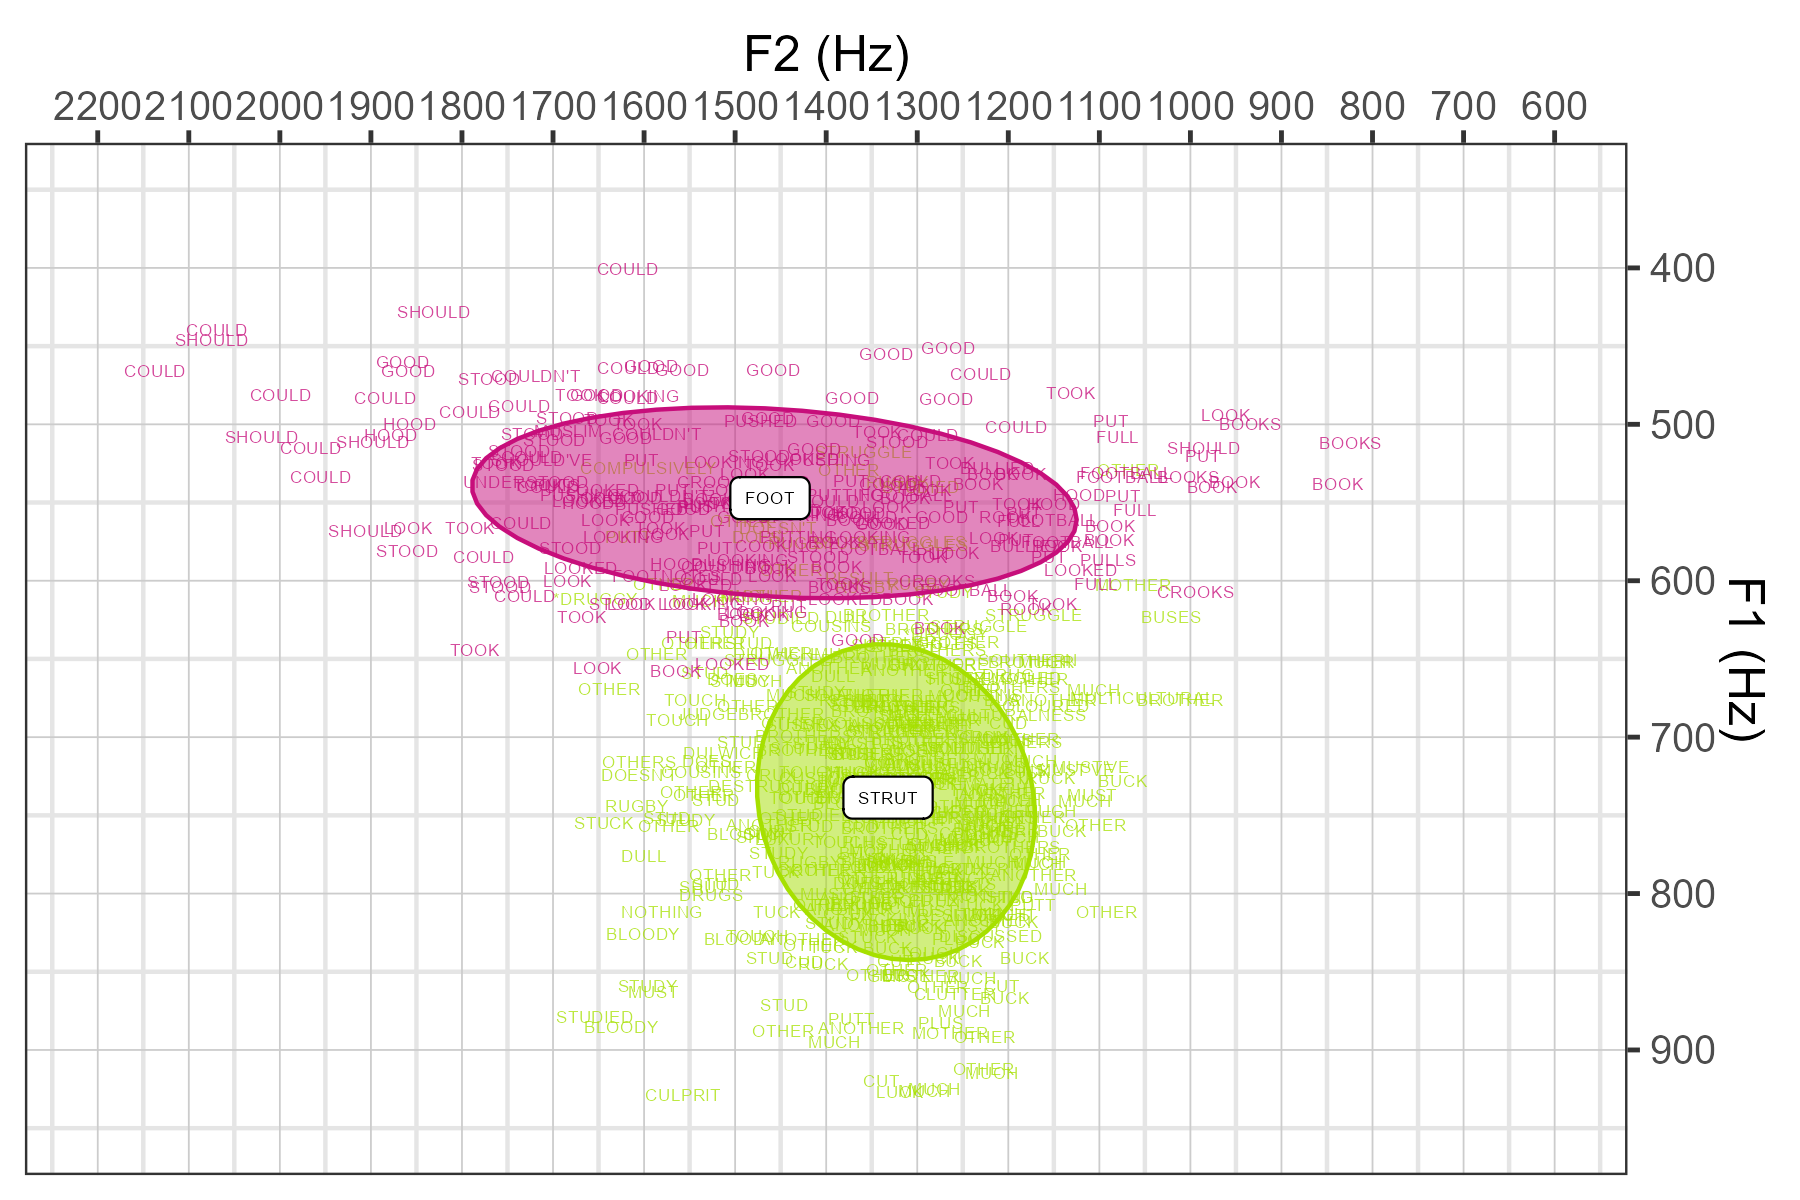
\includegraphics[width=\textwidth]{../figures/FS-SE-vplot.png}
	\caption{Vowel Space plot of \foot{} and \strutt{} in the CoRP-SE speakers} \label{fig:FSvplotSE}
\end{figure}

\subsubsection{F1} \label{subsubsec:SEF1}
The best fit model of the normalised F1 of the \foot{}  and \strutt{}  words is shown in table \ref{tbl:FSF1SE}; the model also includes random intercepts for speaker and word. The model intercept is 536Hz, which is the mean F1 of the \foot{} words. The effect size of lexical Set is +199Hz (t=17.28). Therefore, the mean F1 for the vowels in the \strutt{} words is 735Hz. There is an effect of speaker sex (t=3.77) but the effect size is only 21Hz, which is not large in the context of the lexical set variation. This model demonstrates that the vowels of the two lexical sets are distinct in height in CoRP-SE speakers, with the mean of the \strutt{} lexical set lower in the mouth than the mean of the \foot{} lexical set, by 199Hz. The difference is visualised in figure \ref{fig:FSF1SE} (based on raw data, not the model predictions), where the distinction between the vowel measurements in the two lexical sets can be seen clearly, with no overlap between the interquartile ranges.

% latex table generated in R 4.1.0 by xtable 1.8-4 package
% Thu Nov 11 17:36:55 2021
\begin{table}[ht]
\centering
\begin{tabular}{lrr}
  \hline
fixedeffect & estimate & tvalue \\ 
  \hline
(Intercept) & 536.37 & 35.36 \\ 
  lexSetSTRUT & 199.08 & 17.28 \\ 
  sexSum1 & 20.57 & 3.77 \\ 
  ageGroupSum1 & 3.82 & 0.71 \\ 
  folManSum1 & 12.17 & 0.76 \\ 
  folManSum2 & 0.15 & 0.02 \\ 
  folManSum3 & -20.85 & -1.56 \\ 
  preSeg\_smallSum1 & 19.32 & 1.50 \\ 
  preSeg\_smallSum2 & 11.43 & 1.32 \\ 
  preSeg\_smallSum3 & -12.04 & -0.96 \\ 
  preSeg\_smallSum4 & -19.77 & -0.95 \\ 
  freq.zipf\_z & 0.61 & 0.11 \\ 
  styleSum1 & -16.14 & -2.18 \\ 
  styleSum2 & 7.27 & 0.79 \\ 
  time\_z & 1.55 & 0.43 \\ 
   \hline
\end{tabular}
\caption{Linear Mixed Effects Model of F1 of \textsc{foot} and \textsc{strut} in the South East \label{tbl:FSF1SE}} 
\end{table}


\begin{figure}[h]
	\centering
	\includesvg[width=\textwidth]{../figures/FS-SE-F1.svg}
	\caption{F1 of \foot{} and \strutt{} in CoRP-SE speakers} \label{fig:FSF1SE}
\end{figure}

\subsubsection{F2} \label{subsubsec:SEF2}
Modelling F2 (see table \ref{tbl:FSF2SE}) showed an intercept of 1383Hz, the mean of the \foot() lexical set, and while there is a lot less variation according to lexical set than seen in F1, there is a difference of -86Hz (t =-2.58) implying that the mean of the \strutt{} vowel is slightly further back than the mean of the \foot{} vowel in south-eastern speakers, this can be seen in figure \ref{fig:FSF2SE}. This difference is not large and it can be seen in figure \ref{fig:FSF2SE} that the inter-quartile range is almost completely overlapping; the \strutt{} words sit almost completely within the range of the \foot{} words.
There is also a small but significant effect of style.

% latex table generated in R 4.1.0 by xtable 1.8-4 package
% Thu Nov 11 17:36:56 2021
\begin{table}[ht]
\centering
\begin{tabular}{lrr}
  \hline
fixedeffect & estimate & tvalue \\ 
  \hline
(Intercept) & 1386.41 & 29.16 \\ 
  lexSetSTRUT & -85.98 & -2.58 \\ 
  sexSum1 & -13.82 & -0.56 \\ 
  ageGroupSum1 & -20.93 & -0.84 \\ 
  folManSum1 & 10.77 & 0.23 \\ 
  folManSum2 & -1.30 & -0.05 \\ 
  folManSum3 & -52.11 & -1.37 \\ 
  preSeg\_smallSum1 & -26.20 & -0.69 \\ 
  preSeg\_smallSum2 & -15.12 & -0.60 \\ 
  preSeg\_smallSum3 & -62.95 & -1.74 \\ 
  preSeg\_smallSum4 & 107.84 & 1.81 \\ 
  freq.zipf\_z & -2.61 & -0.17 \\ 
  styleSum1 & 62.19 & 3.24 \\ 
  styleSum2 & -43.60 & -1.88 \\ 
  time\_z & 15.37 & 1.67 \\ 
   \hline
\end{tabular}
\caption{Linear Mixed Effects Model of F2 of \textsc{foot} and \textsc{strut} in the South East \label{tbl:FSF2SE}} 
\end{table}


\begin{figure}[h]
	\includesvg[width=\textwidth]{../figures/FS-SE-F2.svg}
	\caption{F2 of \foot{} and \strutt{} in CoRP-SE speakers} \label{fig:FSF2SE}
\end{figure}

A further model was run including \strutt{}, \scs{thought}, and schwa, to check  the frontness of the \strutt{} vowel of in comparison to other vowels at a similar height in the English vowel space. The model summary can be found in appendix \ref{app:STSEF2}; it shows that the \strutt{} vowel in these speakers is significantly further forward than the \scs{thought} vowel (-399Hz, t=-13.50) and also significantly further back than the schwa (305Hz, t=8.16), placing it between the two in the vowel space, but closer to schwa (see figure \ref{fig:STF2SE}).
`
\begin{figure}[h]
	\includesvg[width=\textwidth]{../figures/ST-SE-F2.svg}
	\caption{F2 of \strutt{}, \scs{thought}, and schwa in CoRP-SE speakers} \label{fig:STF2SE}
\end{figure}



\subsection{DECTE speakers}
Overall, the DECTE speakers do not show a split in height, as measured by F1 and while they show some F2 differences between \foot{} and \strutt{} in the old age group (+147Hz) the pattern is clearly different to that found in the CoRP-SE speakers and it can be concluded that according to this sample, the majority of state-educated speakers in the North East do not show a \FS{} split. Further analysis of the F1 and F2 dimensions is continued below.

\begin{figure}[h]
	\centering
	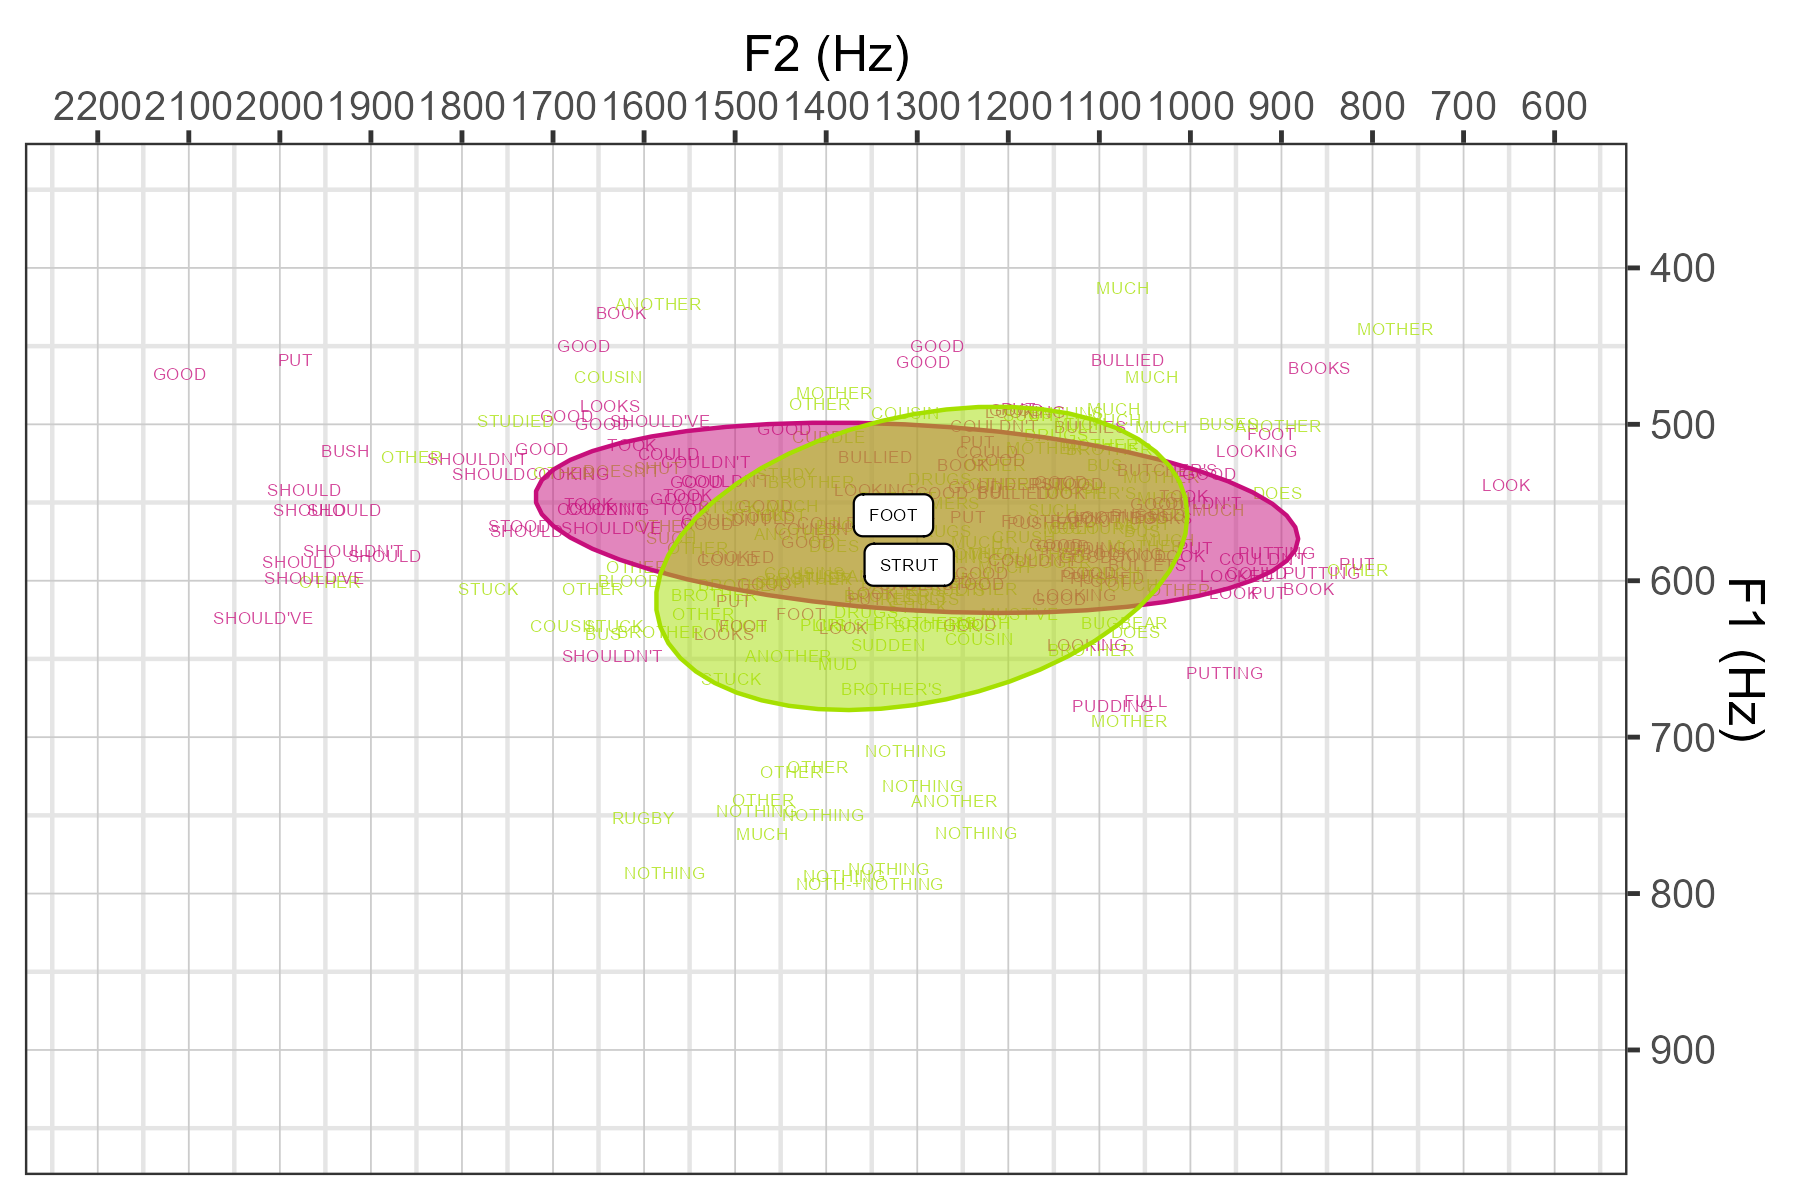
\includegraphics[width=\textwidth]{../figures/FS-DE-vplot.png}
	\caption{Vowel Space plot of \foot{} and \strutt{} in the DECTE speakers} \label{fig:FSvplotDE}
\end{figure}

\subsubsection{F1}
Modelling F1 of the \foot{} and \strutt{} words in the DECTE speakers gives an intercept of 572Hz (table \ref{tbl:FSF1DE}), which is the mean of the \foot{} words, and no significant effect of lexical set (seen in figure \ref{fig:FSF1DE}). However, when looking at individual speakers, as shown in figure \ref{fig:FSF1DE-id}, it does appear that some speakers have a small difference. Since the best fit model did not include random effect for speaker it is not possible to investigate this further.

% latex table generated in R 4.1.0 by xtable 1.8-4 package
% Fri Nov 12 21:59:30 2021
\begin{table}[ht]
\centering
\begin{tabular}{lrr}
  \hline
fixedeffect & estimate & tvalue \\ 
  \hline
(Intercept) & 571.28 & 27.70 \\ 
  lexSetSTRUT & 27.12 & 1.47 \\ 
  sexSum1 & 3.53 & 0.72 \\ 
  ageGroupSum1 & -8.55 & -1.70 \\ 
  folManSum1 & -19.81 & -0.86 \\ 
  folManSum2 & 5.81 & 0.41 \\ 
  folManSum3 & 14.90 & 0.69 \\ 
  preSeg\_smallSum1 & 24.82 & 1.14 \\ 
  preSeg\_smallSum2 & -4.07 & -0.30 \\ 
  preSeg\_smallSum3 & 1.52 & 0.07 \\ 
  preSeg\_smallSum4 & -19.53 & -0.65 \\ 
  freq.zipf\_z & 7.14 & 0.75 \\ 
  time\_z & 11.41 & 1.84 \\ 
   \hline
\end{tabular}
\caption{Linear Mixed Effects Model of F1 of \textsc{foot} and \textsc{strut} in DECTE speakers \label{tbl:FSF1DE}} 
\end{table}


\begin{figure}
	\centering
	\includesvg[width=\textwidth]{../figures/FS-DE-F1.svg}
	\caption{F1 of \foot{} and \strutt{} in DECTE speakers} \label{fig:FSF1DE}
\end{figure}

\begin{figure}
	\centering
	\includesvg[width=\textwidth]{../figures/FS-DE-F1-id.svg}
	\caption{F1 of \foot{} and \strutt{} in DECTE speakers, by speaker} \label{fig:FSF1DE-id}
\end{figure}


\subsubsection{F2}
The best fit model of F2 of the \foot{} and \strutt{} words in the DECTE speakers (table \ref{tbl:FSF2DE}) includes an interaction of lexical set and age group. The intercept (mean of \foot{} words in old speakers) is 1232Hz, the mean of \foot{} words in young speakers is 1638Hz. The split in the old age group is +147Hz whereas in the young age group it is -26Hz. It is possible that the split in the younger speakers is affected by the  fronting of \foot{} due to the Tyneside phenomenon of \foot{} merging with \goose{}, which seems to be more prevalent in the younger speakers in this age group (figure \ref{fig:FSGF2DE-age})\todoreference{find a reference}.


% latex table generated in R 4.1.0 by xtable 1.8-4 package
% Thu Nov 11 17:37:02 2021
\begin{table}[ht]
\centering
\begin{tabular}{lrr}
  \hline
fixedeffect & estimate & tvalue \\ 
  \hline
(Intercept) & 1232.05 & 19.07 \\ 
  lexSetSTRUT & 146.67 & 2.67 \\ 
  ageGroupYoung & 405.58 & 6.41 \\ 
  sexSum1 & -48.29 & -1.80 \\ 
  folManSum1 & -73.52 & -1.13 \\ 
  folManSum2 & -12.44 & -0.31 \\ 
  folManSum3 & 11.04 & 0.18 \\ 
  preSeg\_smallSum1 & -150.48 & -2.42 \\ 
  preSeg\_smallSum2 & -139.84 & -3.60 \\ 
  preSeg\_smallSum3 & -148.60 & -2.36 \\ 
  preSeg\_smallSum4 & 458.85 & 5.36 \\ 
  freq.zipf\_z & 25.87 & 0.95 \\ 
  time\_z & -37.39 & -1.96 \\ 
  lexSetSTRUT:ageGroupYoung & -172.85 & -2.88 \\ 
   \hline
\end{tabular}
\caption{Linear Mixed Effects Model of F2 of \textsc{foot} and \textsc{strut} in DECTE speakers \label{tbl:FSF2DE}} 
\end{table}


\begin{figure}
	\centering
	\includesvg[width=\textwidth]{../figures/FSG-DE-F2-age.svg}
	\caption{F2 of \foot{}, \strutt{}, and \goose{} in DECTE speakers, by age group} \label{fig:FSGF2DE-age}
\end{figure}


\subsection{CoRP-NE speakers} \label{subsec:FSNE}
CoRP-NE speakers show some evidence of a \FS{} split, particularly in F1 (on average 110Hz, higher in female speakers) but little evidence of an F2 split except in one speaker. Further analysis of the F1 and F2 differences can be seen below, but from the vowel space plot in figure it can be seen that the \strutt{} words are lower than the \foot{} words (with some overlap) but have similar frontness.

\begin{figure}[h]
	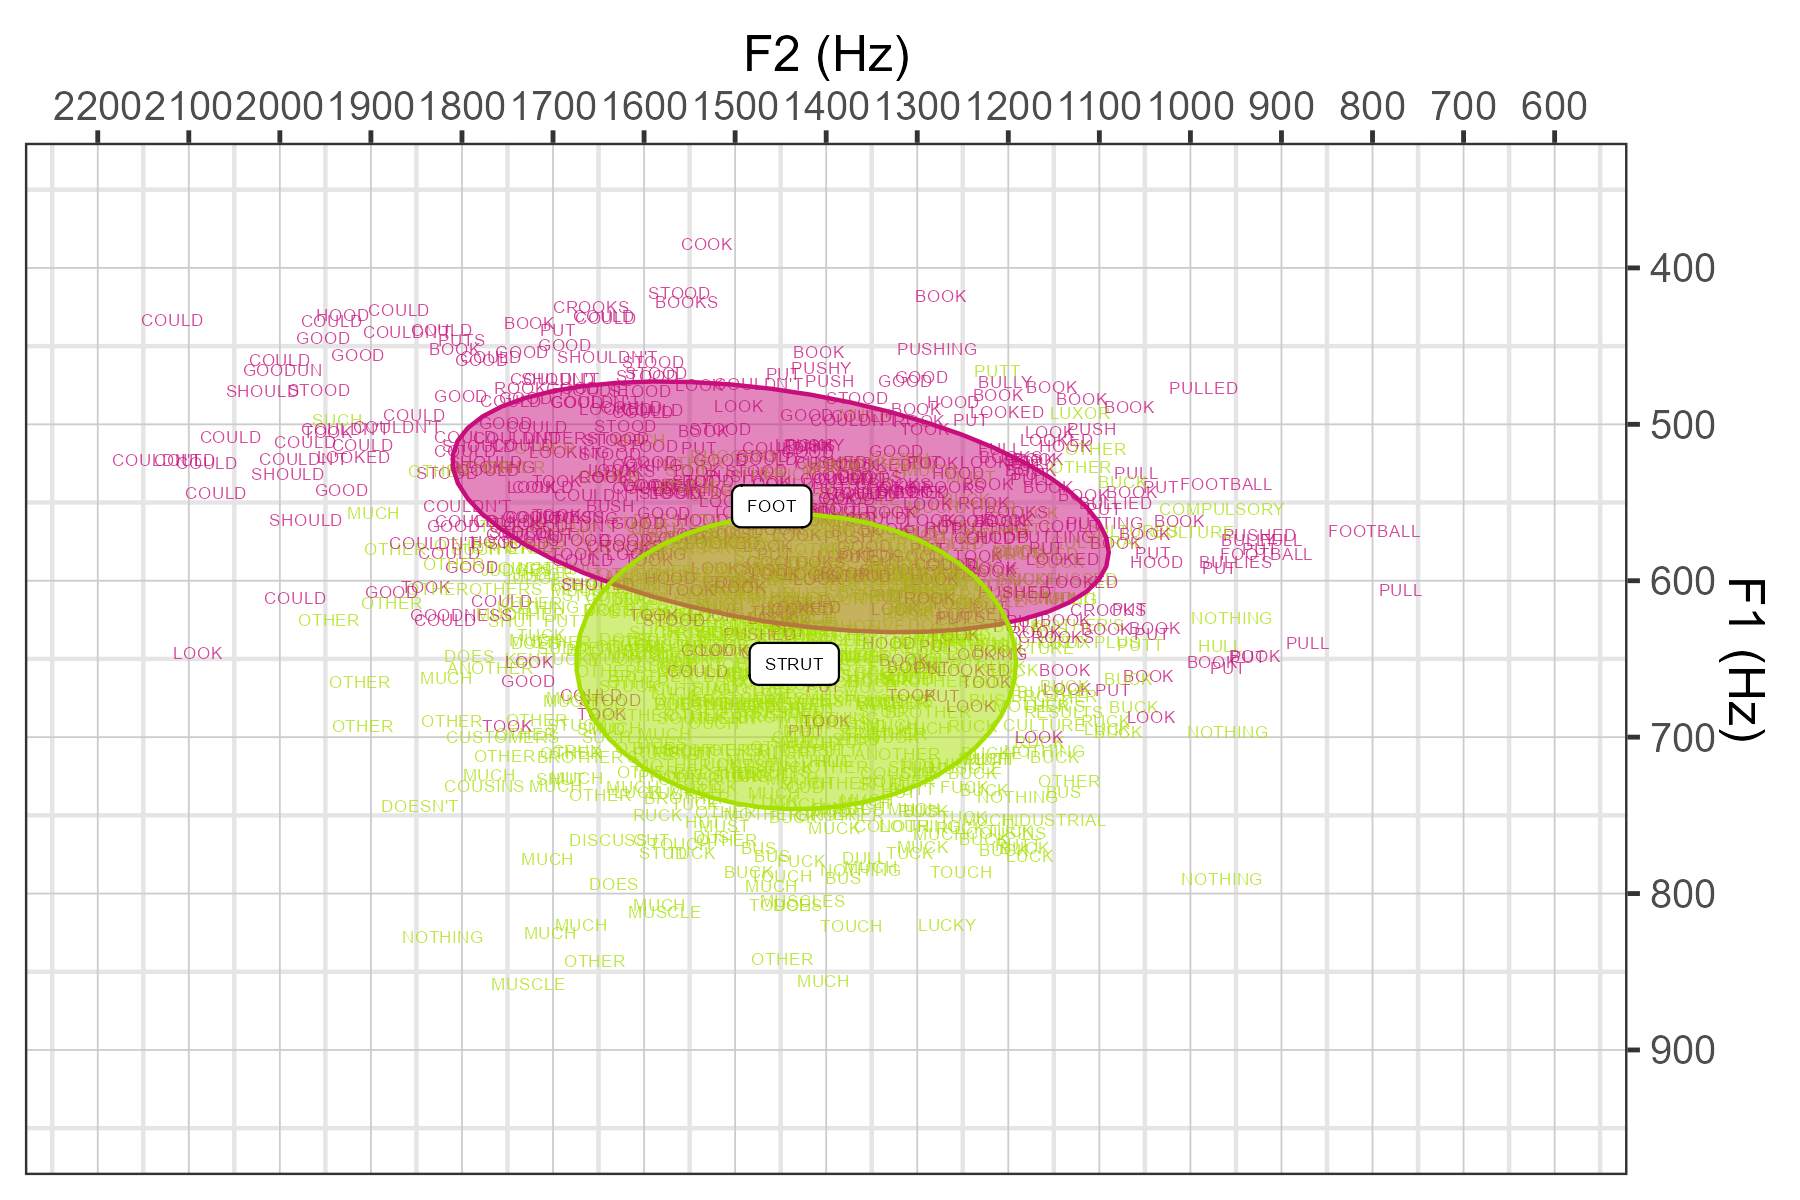
\includegraphics[width=\textwidth]{../figures/FS-NE-vplot.png}
	\caption{Vowel Space plot of \foot{} and \strutt{}, in the CoRP-NE speakers} \label{fig:FSvplotNE}
\end{figure}


\subsubsection{F1} \label{subsubsec:NEF1}

The best fit model for F1 of the CoRP-NE speakers can be seen in table \ref{tbl:FSF1NE} and shows a \FS{} split in F1 that interacts with both speaker sex and age group. The mean value of \foot{} is 541.53 and the mean value of \strutt{} is 651Hz, showing an average split of 110Hz. However, this split is overall higher for female speakers (mean=142Hz) compared to male speakers (mean=78Hz) (64 Hz difference), there is also a slightly larger split in older speakers. Overall the size of split is ranked: old female, young female, old male, young male.

% latex table generated in R 4.1.0 by xtable 1.8-4 package
% Thu Nov 11 17:36:59 2021
\begin{table}[ht]
\centering
\begin{tabular}{lrr}
  \hline
fixedeffect & estimate & tvalue \\ 
  \hline
(Intercept) & 516.30 & 27.03 \\ 
  lexSetSTRUT & 172.92 & 14.45 \\ 
  sexMale & 32.17 & 1.22 \\ 
  ageGroupYoung & 36.03 & 1.88 \\ 
  folManSum1 & -12.31 & -1.08 \\ 
  folManSum2 & 11.62 & 1.59 \\ 
  folManSum3 & -5.03 & -0.52 \\ 
  preSeg\_smallSum1 & 24.05 & 2.49 \\ 
  preSeg\_smallSum2 & 12.59 & 1.82 \\ 
  preSeg\_smallSum3 & -22.43 & -2.08 \\ 
  preSeg\_smallSum4 & -9.66 & -0.56 \\ 
  freq.zipf\_z & 2.55 & 0.61 \\ 
  styleSum1 & -12.35 & -2.17 \\ 
  styleSum2 & 5.40 & 0.78 \\ 
  lexSetSTRUT:sexMale & -89.79 & -5.32 \\ 
  lexSetSTRUT:ageGroupYoung & -61.66 & -5.40 \\ 
  sexMale:ageGroupYoung & -36.95 & -1.18 \\ 
  lexSetSTRUT:sexMale:ageGroupYoung & 50.89 & 2.53 \\ 
   \hline
\end{tabular}
\caption{Linear Mixed Effects Model of F1 of \textsc{foot} and \textsc{strut} in the North East \label{tbl:FSF1NE}} 
\end{table}


% Table generated by Excel2LaTeX from sheet 'Sheet1'
% Table generated by Excel2LaTeX from sheet 'FS-NE-F1-lexSet-sex-ageGroup'
\begin{table}[htbp]
	\centering
	\begin{tabular}{lrrr}
		\hline
		& \multicolumn{1}{l}{\foot{}} & \multicolumn{1}{l}{\strutt{}} & \multicolumn{1}{l}{\textit{size of split}} \\
		\hline
		Old Female & 516.3 & 689.22 & \textit{172.92} \\
		Old Male & 548.47 & 631.6 & \textit{83.13} \\
		Young Female & 553.07 & 664.33 & \textit{111.26} \\
		Young Male & 548.29 & 620.65 & \textit{72.36} \\
		Mean  & 541.53 & 651.45 & \textit{109.92} \\
		\hline
	\end{tabular}%
	\caption{table showing interactions effects of speaker age group and sex on F1 of \foot{} and \strutt{} in CoRP-NE speakers (calculated from interactions in table \ref{tbl:FSF1NE})}
	\label{tbl:FSF1NEinter}%
\end{table}%

\begin{figure}[h]
	\includesvg[width=\textwidth]{../figures/FS-NE-F1.svg}
	\caption{F1 of \foot{} and \strutt{} in CoRP-NE speakers} \label{fig:FSF1NE}
\end{figure}


\subsubsection{F2} \label{subsubsec:NEF2}
The best fit model for F2 of the CoRP-NE speakers (see table \ref{tbl:FSF2NE}) also includes a three way interaction between lexical set, sex, and age group (summarised in figure \ref{tbl:FSF2NEinter}). The mean value of \foot{} is 1339Hz and the mean value of \strutt{} is 1380Hz, showing very little distinction, when the interaction is considered the largest distinction that is seen is in the opposite direction to the CoRP-SE speakers showing a \strutt{} vowel that is slightly fronter than the \foot{} vowel.

% latex table generated in R 4.1.0 by xtable 1.8-4 package
% Fri Nov 12 10:49:26 2021
\begin{table}[ht]
\centering
\begin{tabular}{lrr}
  \hline
fixedeffect & estimate & tvalue \\ 
  \hline
(Intercept) & 1468.01 & 25.11 \\ 
  lexSetSTRUT & -27.34 & -0.68 \\ 
  sexMale & -261.86 & -3.42 \\ 
  ageGroupYoung & -77.10 & -1.45 \\ 
  folManSum1 & 81.82 & 1.71 \\ 
  folManSum2 & 52.98 & 1.89 \\ 
  folManSum3 & -209.68 & -5.95 \\ 
  preSeg\_smallSum1 & -45.91 & -1.21 \\ 
  preSeg\_smallSum2 & -28.81 & -1.10 \\ 
  preSeg\_smallSum3 & -68.50 & -1.71 \\ 
  preSeg\_smallSum4 & 161.72 & 2.57 \\ 
  freq.zipf\_z & 28.41 & 1.74 \\ 
  styleSum1 & 56.67 & 3.08 \\ 
  styleSum2 & -30.87 & -1.52 \\ 
  time\_z & -6.79 & -0.83 \\ 
  lexSetSTRUT:sexMale & 203.82 & 4.34 \\ 
  lexSetSTRUT:ageGroupYoung & 52.55 & 1.67 \\ 
  sexMale:ageGroupYoung & 162.76 & 1.84 \\ 
  lexSetSTRUT:sexMale:ageGroupYoung & -240.35 & -4.31 \\ 
   \hline
\end{tabular}
\caption{Linear Mixed Effects Model of F2 of \textsc{foot} and \textsc{strut} in the North East \label{tbl:FSF2NE}} 
\end{table}


% Table generated by Excel2LaTeX from sheet 'FS-NE-F2-lexSet-sex-ageGroup'
\begin{table}[htbp]
	\centering
	\begin{tabular}{lrrr}
		\hline
		& \multicolumn{1}{l}{\foot{}} & \multicolumn{1}{l}{\strutt{}} & \multicolumn{1}{l}{\textit{size of split}} \\
		\hline
		Old Female & 1468.01 & 1440.67 & \textit{-27.34} \\
		Old Male & 1206.15 & 1382.63 & \textit{176.48} \\
		Young Female & 1390.91 & 1416.12 & \textit{25.21} \\
		Young Male & 1291.81 & 1280.49 & \textit{-11.32} \\
		Mean  & 1339.22 & 1379.98 & \textit{40.76} \\
		\hline
	\end{tabular}%
	\caption{table showing effects of speaker age group and sex on F2 of \foot{} and \strutt{} in CoRP-NE speakers (calculated from table \ref{tbl:FSF2NE})}
	\label{tbl:FSF2NEinter}
	\end{table}%


\subsection{Conclusions on the nature of the \FS{} Split in all three speaker groups}
In the CoRP-SE speakers the \foot{} and \strutt{} vowel are distinguished in F1 (a difference of +110Hz) and F2 (-86Hz). The F1 difference is clearly meaningful but while the F2 difference is present and statistically significant it needs to be considered more carefully because it is only a small difference within the whole vowel space. Overall the \FS split can be described as mostly characterised by height and slightly by frontness. It was also found that the frontness of the \strutt{} vowel in the South East is between the schwa and \scs{thought} vowels, but closer to schwa. If the CoRP-NE speakers are behaving like the CoRP-SE speakers, we would expect them to have a similar pattern in both F1 and possibly F2.

In the DECTE speakers we see what can be considered \quotesingle{normal} North East \FS{} positions of \foot{} and \strutt{}. The speakers show no significant difference between \foot{} and \strutt{} in F1, and in F2 a small difference in mainly older speakers (+147Hz). It can be concluded that there is not a robust \FS{} split in the North East as found in the CoRP-SE speakers.

In CoRP-NE speakers we some evidence of a split. They show an F1 difference of 110Hz (mean, male and female speakers behave differently) and some F2 difference in the opposite direction to CoRP-SE. This suggests that these speakers have a split, but it is not identical to the split found in the CoRP-SE speakers. It is not as large in height (F1 is 110Hz vs the 199Hz found in CoRP-SE speakers) and does not seem to exist in frontness.

By analysis of the \foot{} and \strutt{} words in all three speaker groups it can be concluded that CoRP-NE speakers do not behave identically to either of the other speaker groups. However, conclusions can be drawn in answer to research question \onlyinsubfile{1}\notinsubfile{\ref{RQ1}}. The DECTE speakers (state educated in the North East) do not show any \FS{} split and CoRP-NE speakers clearly have at least some distinction between \foot{} and \strutt{} so it can be concluded that they are not behaving consistently regionally. While the CoRP-NE speakers do not show as large a split as the CoRP-SE speakers, there is clearly a split present, demonstrating at least a tendency towards non-regional behaviour.

In order to further understand the nature of the difference between the split in different speaker groups the \strutt{} words were modelled separately, results of this are discussed in section \ref{sec:FSSTRUT}.

\section{\scs{Strut vowel only}} \label{sec:FSSTRUT}
\subsection{F1}
% latex table generated in R 4.1.0 by xtable 1.8-4 package
% Tue Nov 16 11:46:14 2021
\begin{table}[ht]
\centering
\begin{tabular}{lrr}
  \hline
fixedeffect & estimate & tvalue \\ 
  \hline
(Intercept) & 671.04 & 43.85 \\ 
  relevel(corpus, "CoRP-NE")DECTE-NE & -79.47 & -5.16 \\ 
  relevel(corpus, "CoRP-NE")CoRP-SE & 93.87 & 6.42 \\ 
  sexMale & -47.85 & -3.41 \\ 
  ageGroupSum1 & 3.91 & 0.76 \\ 
  folManSum1 & -3.69 & -0.25 \\ 
  folManSum2 & 12.89 & 1.48 \\ 
  folManSum3 & -21.14 & -1.79 \\ 
  preSeg\_smallSum1 & 12.66 & 0.86 \\ 
  preSeg\_smallSum2 & 15.56 & 1.72 \\ 
  preSeg\_smallSum3 & -17.46 & -1.47 \\ 
  preSeg\_smallSum4 & -21.44 & -0.93 \\ 
  freq.zipf\_z & 6.54 & 1.06 \\ 
  styleSum1 & -20.18 & -2.28 \\ 
  styleSum2 & 14.45 & 1.48 \\ 
  relevel(corpus, "CoRP-NE")DECTE-NE:sexMale & 77.98 & 3.00 \\ 
  relevel(corpus, "CoRP-NE")CoRP-SE:sexMale & 4.27 & 0.19 \\ 
   \hline
\end{tabular}
\caption{Linear Mixed Effects Model of F1 of \textsc{strut} \label{tbl:strutF1}} 
\end{table}

Modelling the \strutt{} vowel alone (see table \ref{tbl:strutF1}) shows that the CoRP-NE speakers are significantly different in F1 from both the CoRP-SE and the DECTE speakers. The best fit model included an interaction between corpus and speaker sex, the results of which are shown in table \ref{tbl:strutF1inter}. These results partially support those above but add an extra dimension. The mean F1 value for \strutt{} in CoRP-NE female speakers is between the CoRP-SE and DECTE values, but the male speakers show a vowel that is very similar to the DECTE speakers (visualised in figure \ref{fig:strutF1-sex}). This implies that while female speakers are not behaving regionally, male speakers are.

% Table generated by Excel2LaTeX from sheet 'strut corpus-sex'
\begin{table}[htbp]
	\centering
	\begin{tabular}{lrrr}
		\hline
		& \multicolumn{1}{l}{CoRP-SE} & \multicolumn{1}{l}{DECTE} & \multicolumn{1}{l}{CoRP-NE} \\
		\hline
		Female & 764.91 & 591.57 & 671.04 \\
		Male  & 721.78 & 621.7 & 623.19 \\
		\textit{Mean} & \textit{743.35} & \textit{606.64} & \textit{647.12} \\
		\hline
	\end{tabular}%
	\caption{table showing effects of corpus group and speaker sex on F1 of \strutt{} (calculated from table \ref{tbl:strutF1})}
	\label{tbl:strutF1inter}%
\end{table}%

\begin{figure}[h]
	\includesvg[width=\textwidth]{../figures/strut-F1-sex.svg}
	\caption{F1 of \strutt{} in CoRP-SE, DECTE, and CoRP-NE speakers, by speaker sex} \label{fig:strutF1-sex}
\end{figure}


\subsection{F2}
Modelling F2 of the \strutt{} words alone again shows an interaction of corpus and speaker sex (\ref{tbl:strutF2}). In each corpus the male speakers have a less front vowel, and overall the CoRP-NE speakers have the most front vowel, in both male and female speakers. Even if the CoRP-SE vowel is taken as the prototypical \strutt{} vowel there is variation between male and female, with male speakers producing a less front vowel (82Hz difference). The DECTE speakers show a relatively similar frontness to the CoRP-SE speakers, however the CoRP-NE speakers behave differently, both male and female speakers produce a fronter \strutt{} vowel than either of DECTE or CoRP-SE speakers, though the female difference is larger (see tables \ref{tbl:strutF2} and \ref{tbl:strutF2-inter}).
% latex table generated in R 4.1.0 by xtable 1.8-4 package
% Thu Nov 11 17:37:06 2021
\begin{table}[ht]
\centering
\begin{tabular}{lrr}
  \hline
fixedeffect & estimate & tvalue \\ 
  \hline
(Intercept) & 1432.78 & 19.02 \\ 
  relevel(corpus, "CoRP-NE")DECTE-NE & -57.45 & -1.14 \\ 
  relevel(corpus, "CoRP-NE")CoRP-SE & -85.31 & -1.67 \\ 
  sexMale & -15.36 & -0.38 \\ 
  ageGroupYoung & 24.43 & 0.57 \\ 
  folManfricative & -36.83 & -0.76 \\ 
  folManlateral & -169.04 & -3.02 \\ 
  folManstop & -43.68 & -0.87 \\ 
  preSeg\_smallstop & 33.96 & 0.83 \\ 
  preSeg\_smallobstruent-liquid & 2.89 & 0.06 \\ 
  preSeg\_smallSH/JH & 185.52 & 2.45 \\ 
  preSeg\_smallnone & 56.13 & 0.95 \\ 
  freq.zipf\_z & 12.17 & 0.84 \\ 
  styleminimalpair & -29.86 & -0.76 \\ 
  stylewordlist & -10.90 & -0.38 \\ 
  time\_z & 1.94 & 0.32 \\ 
   \hline
\end{tabular}
\caption{Linear Mixed Effects Model of F2 of \textsc{strut} \label{tbl:SF2}} 
\end{table}


% Table generated by Excel2LaTeX from sheet 'strut-F2 corpus-sex'
\begin{table}[htbp]
	\centering
	\begin{tabular}{lrrr}
		\hline
		& \multicolumn{1}{l}{CoRP-SE} & \multicolumn{1}{l}{DECTE} & \multicolumn{1}{l}{CoRP-NE} \\
		\hline
		Female & 1308.8 & 1327.07 & 1476.1 \\
		Male  & 1226.93 & 1263.47 & 1353.37 \\
		\textit{Mean} & \textit{1267.87} & \textit{1295.27} & \textit{1414.74} \\
		\hline
	\end{tabular}%
	\caption{table showing effects of corpus on F2 of \strutt{} (calculated from interaction effects in table \ref{tbl:strutF2})}
	\label{tbl:strutF2-inter}%
\end{table}%


\begin{figure}[h]
	\includesvg[width=\textwidth]{../figures/strut-F2-sex.svg}
	\caption{} \label{fig:strutF2-sex}
\end{figure}

\section{Discussion \& Conclusion}
Modelling the behaviour of both \foot{} and \strutt{} in section \ref{sec:FSSplit} showed that the \FS{} split is mostly characterised by a difference in height, though some evidence of a frontness difference is found. The CoRP-NE speakers were found to have some evidence of a \FS{} split, the difference between the two lexical sets was larger than in the DECTE speakers but smaller than in the CoRP-SE speakers. Further analysis of the \strutt{} vowel alone showed that this difference is mainly due to the female speakers. The majority of male speakers seem to maintain the local pattern found in the DECTE speakers. The F2 pattern is a little more complex and likely is less informative when it comes to behaviour of the \FS{} split. As stated above, there is only some evidence of a split in frontness in the CoRP-SE speakers, who only show a difference of -86Hz, which is not a large change in frontness. In the focussed analysis of \strutt{} alone it can be seen that the CoRP-NE speakers have a different F2 to both the DECTE and CoRP-SE speakers. This shows that their production of the \strut{} vowel, particularly in the female speakers is diverging from both groups.

There are two factors that need to be considered in relation to the results described above.
First, the differences between privately educated and state-educated speakers as a type of social class variation, since while it is not occupation based, it is a form of social stratification connected to income, education and other social opportunities (see chapter \onlyinsubfile{3}\notinsubfile{\ref{ch:LitReviewSocio}} for further discussion of this approach). It is a known effect that male and female speakers diverge in socially stratified accent variation \citep{Labov2001b}, and this effect has been specifically attested in Newcastle \citep{Watt1998}. In general it has been seen that female speakers tend towards a standard and local variants are more often found in male speakers (for example the Tyneside centring diphthongs in \goat{} and \scs{face} are found in male working class speakers by \cite{Watt1998}). The pattern we see in the CoRP-NE speakers where male speakers have a \strutt{} vowel that is similar to the DECTE speakers whereas female speakers have a \strutt{} vowel that is different to them and more similar to the CoRP-SE speakers, clearly reflects this tendency. Male speakers are producing a local variant (though local here is likely \quotesingle{northern} rather than Tyneside specific) and female speakers are tending towards a non-local variant.

Secondly, while the CoRP-NE female speakers discussed above do seem to tend towards a southern-like \strutt{} vowel, they do not successfully reach the target. The F1 is lower than in the CoRP-SE speakers and the F2 is slightly higher. This difference may be the source of a the description occasinoally given to \strutt{} realisations found in the north as \quotesingle{schwa-like} \citep{Braber2015,Jansen2020}\todocontent{include graph or is that overkill?}. It is possible that the speakers are creating a different target for the \strutt{} vowel but it is also possible that they are aiming for the target as realised by CoRP-SE and other southern speakers but not hitting it. Not being able to reach the target could be be due to later acquisition of the split \citep{Evans2007} , but this is difficult to determine with the data available. While information on parent's education and region was collected, there are not enough speakers to draw meaningful conclusions. Another approach to understanding this would be to record people still at school (at various stages) to see when the \FS{} split appears in their speech.

Further discussion on the implications of the variation found here will be undertaken in chapter \onlyinsubfile{9}\notinsubfile{\ref{ch:Discussion}}.




\onlyinsubfile{
	
	\pagebreak
	\listoftodos{}
	\pagebreak
	\bibliography{../../../References/methodology,
					../../../References/footStrut,
					../../../References/tynesideEnglish
		}
			
\appendix
\section{Extra models}
\subsection{F2 of \strutt{} and \scs{thought} in the CoRP-SE speakers} \label{app:STSEF2}
% latex table generated in R 4.1.0 by xtable 1.8-4 package
% Fri Nov 12 23:15:56 2021
\begin{table}[ht]
\centering
\begin{tabular}{lrr}
  \hline
fixedeffect & estimate & tvalue \\ 
  \hline
(Intercept) & 1296.45 & 37.71 \\ 
  lexSetTHOUGHT & -399.00 & -13.50 \\ 
  lexSetschwa & 305.19 & 8.16 \\ 
  sexSum1 & -12.72 & -0.77 \\ 
  ageGroupSum1 & -4.21 & -0.26 \\ 
  folManSum1 & 37.03 & 0.98 \\ 
  folManSum2 & 17.13 & 0.86 \\ 
  folManSum3 & -102.64 & -5.05 \\ 
  preSeg\_smallSum1 & -55.23 & -1.80 \\ 
  preSeg\_smallSum2 & -16.17 & -0.92 \\ 
  preSeg\_smallSum3 & -69.59 & -2.41 \\ 
  preSeg\_smallSum4 & 68.11 & 1.52 \\ 
  freq.zipf\_z & -1.90 & -0.16 \\ 
  styleSum1 & 59.22 & 3.20 \\ 
  styleSum2 & -47.13 & -2.04 \\ 
   \hline
\end{tabular}
\caption{Linear Mixed Effects Model of F2 of \textsc{strut}, \textsc{thought}, and schwa in the South East \label{tbl:STF2SE}} 
\end{table}


			}

\end{document} 